% 2012 年安徽卷文科第 19 题：长方体 ABCD-A1B1C1D1，O 为 BD 中点，E 在 AA1 上。
% 来源 PDF：普通高考/2012/2012安徽文.pdf，第 2 页（印面 716）第 1 栏。
% 斜二测投影：screen(x,y,z) = (x + 0.5y, z + 0.35y)，底面边长 2、高 3√2 ≈ 4.24 量纲。
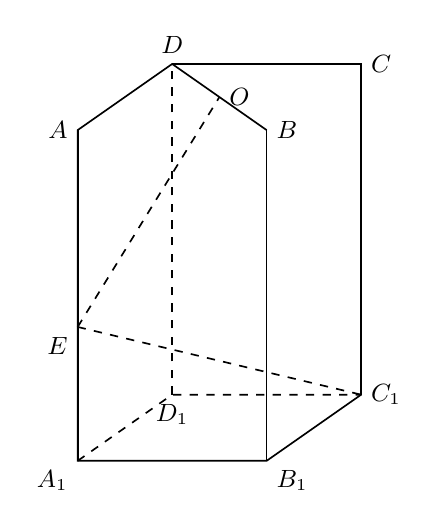
\begin{tikzpicture}[semithick, font=\small]
  % 顶点（x 向右、y 向里、z 向上）
  \coordinate (A1) at (0,0);
  \coordinate (B1) at (2.4,0);
  \coordinate (C1) at (3.6,0.84);
  \coordinate (D1) at (1.2,0.84);
  \coordinate (A)  at (0,4.2);
  \coordinate (B)  at (2.4,4.2);
  \coordinate (C)  at (3.6,5.04);
  \coordinate (D)  at (1.2,5.04);
  \coordinate (O)  at (1.8,4.62);
  \coordinate (E)  at (0,1.7);
  % 实线
  \draw (A1) -- (B1) -- (C1) -- (C) -- (D) -- (A) -- cycle;
  \draw (A1) -- (A);
  \draw (B1) -- (B);
  \draw (C1) -- (C);
  \draw (B) -- (D);
  % 虚线
  \draw[dashed] (A1) -- (D1) -- (C1);
  \draw[dashed] (D1) -- (D);
  \draw[dashed] (E) -- (C1);
  \draw[dashed] (E) -- (O);
  % 标注
  \node[below left] at (A1) {$A_1$};
  \node[below right] at (B1) {$B_1$};
  \node[right] at (C1) {$C_1$};
  \node[below] at (D1) {$D_1$};
  \node[left] at (A) {$A$};
  \node[right] at (B) {$B$};
  \node[right] at (C) {$C$};
  \node[above] at (D) {$D$};
  \node[below left] at (E) {$E$};
  \node[right] at (O) {$O$};
\end{tikzpicture}
